\documentclass[a4paper]{article}
\usepackage[left=3cm, right=3cm]{geometry}
\usepackage{amsmath}
\usepackage{amssymb}
\usepackage{subfigure}
\usepackage{listings}
\usepackage[]{minted}
\usepackage{graphicx}
\usepackage{epstopdf}

\begin{document}

\section{Introduction}

\subsection{Installation and running}

When installing MathGL there are some things to note:
\begin{enumerate}
  \item{You must make sure the dynamic linker finds the MathGL library \\
    (under Linux: add \texttt{export LD\_LIBRARY\_PATH=/usr/local/lib} to your \texttt{$\mathtt{\sim}$/.bashrc})}
    \item{MathGL only works with the GNU Standard. So compile with \texttt{g++}, add the flag \texttt{-std=gnu++11} or add: \\
      \texttt{set(CMAKE\_CXX\_COMPILER /usr/bin/g++) \\
              set(CMAKE\_C\_COMPILER /usr/bin/gcc)} \\
      to your \texttt{CMakeLists.txt}. \\
      Additionally when using the Clang compiler make sure you have the OpenMP library (\texttt{omp.h}). 
      If you already the GNU Compiler you can copy \& paste it from \texttt{gcc}'s includes to \texttt{clang}'s includes.}
  \item{When using with Eigen there are some incompatibilites due to the usage of C-libraries in MathGL,
      so you have to modify your \texttt{mgl2/config.h} by changing: \\
    \texttt{MGL\_HAVE\_C99\_COMPLEX 1} to \texttt{MGL\_HAVE\_C99\_COMPLEX 0}}
\end{enumerate}
When compiling the code then simply add the \texttt{-lmgl} flag. \\
With GNU: \texttt{g++ -lmgl test.cpp} \\ 
With Clang: \texttt{clang++ -lmgl -std=gnu++11 test.cpp} \\

\subsection{Comparison to \textsc{Matlab}}

Most of the \textsc{Matlab} function regarding plotting have an MathGL equivalent. 
The implementation is usually just a few lines longer.
For more detailed information see ``translator.pdf'' or the example-codes below.

\subsection{Plotting runtimes}

Here a small experiment on how fast MathGL is: 
\begin{figure}[h]
  \centering
  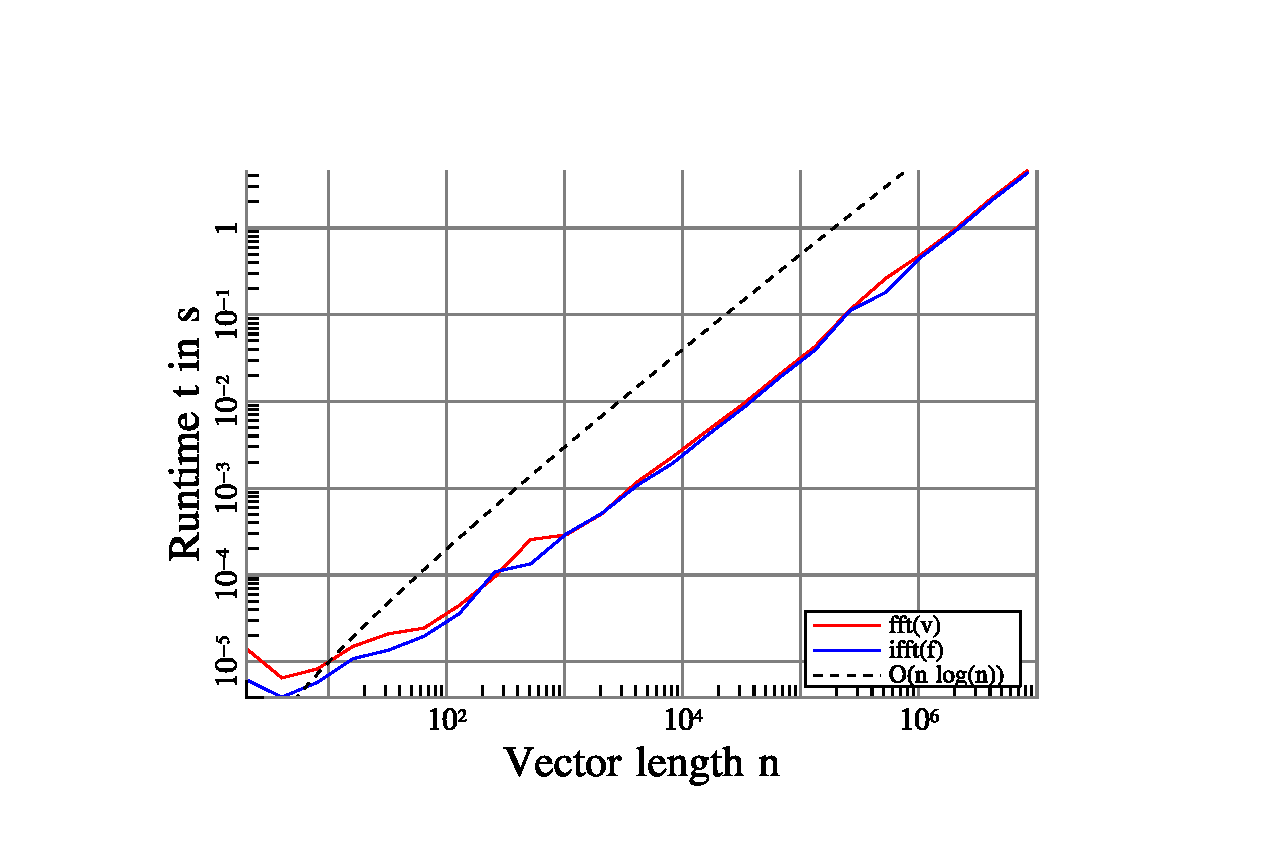
\includegraphics[width=0.6\textwidth]{../../plot-runtime/runtimes.eps}
\end{figure}

\section{Usage with Eigen}

\subsection{Polynomial evaluation}

This example compares naive polynomial evaluation to evaluation with the horner scheme. 
\begin{figure}[h]
  \subfigure[No optimization]{\includegraphics[width=0.5\textwidth]{../../polyeval/runtimes-optimized.eps}}
  \subfigure[With \text{O3} optimization]{\includegraphics[width=0.5\textwidth]{../../polyeval/runtimes-optimized.eps}}
  \caption{Note the order of magnitude difference in the runtimes}
\end{figure}

Code:
\begin{minted}[mathescape,linenos,fontsize=\footnotesize]{c++}
# include <iostream>
# include <chrono>
# include <mgl2/mgl.h>
# include <Eigen/Dense>

using std::chrono::high_resolution_clock;
using std::chrono::nanoseconds;
using std::chrono::duration_cast;

using Eigen::VectorXd;

template <typename Scalar1, typename Scalar2>
void print_pair(std::pair<Scalar1, Scalar2> p){
  std::cout << "( " << p.first << ", " << p.second << " )\n";
}

template <typename Scalar>
Scalar pow(Scalar x, int n){
  Scalar res = x;
  for (int i = 1; i < n; ++i)
    res *= x;
  return res;
}

template <typename Scalar, typename CoeffVec>
Scalar hornerEval(const CoeffVec& c, const Scalar x){
  Scalar res = c(0);
  for (int i = 1; i < c.size(); ++i)
    res = x*res + c(i);
  return res;
}

template <typename Scalar, typename CoeffVec>
Scalar naiveEval(const CoeffVec& c, const Scalar x, bool superbad = true){
  Scalar res = 0;
  if (superbad){
    for (int i = c.size() - 1; i >= 1; --i)
      res += c(i)*pow(x, i);
  }
  else {
    for (int i = c.size() - 1; i >= 1; --i)
      res += c(i)*std::pow(x, i);
  }
  return res;
}

int main(){
  double x = 0.123;
  const unsigned int N = 100000;
  const unsigned int repeats = 1;

  std::vector<double> evals, horner, naive, supernaive;
  evals.reserve(N);
  horner.reserve(N);
  naive.reserve(N);
  supernaive.reserve(N);

  // testing for: horner scheme - naive with naive power-function
  // - naive with efficient power function
  for (unsigned int d = 2; d < N; d *=2){
    Eigen::VectorXd c(d);
    for (unsigned int i = 0; i < d; ++i)
      c(i) = i + 1;
    // saving degrees for which we evaluated
    evals.push_back(d);
    double buffer;

    // horner scheme
    auto ht = high_resolution_clock::now();
    for (unsigned int i = 0; i < repeats; ++i)
      buffer = hornerEval(c, x);
    horner.push_back(duration_cast<nanoseconds>(high_resolution_clock::now() -
    ht).count()/double(1e9)); // normalize data to seconds
    std::cout << buffer; // to make sure the loop doesnt get optimized away
    
    // naive evaluation with naive power function     
    auto nt = high_resolution_clock::now();
    for (unsigned int i = 0; i < repeats; ++i)
      buffer = naiveEval(c, x);
    supernaive.push_back(duration_cast<nanoseconds>(high_resolution_clock::now() - 
    nt).count()/double(1e9));
    std::cout << buffer;
    
    // naive evaluation with std::pow
    auto nt2 = high_resolution_clock::now();
    for (unsigned int i = 0; i < repeats; ++i)
      buffer = naiveEval(c, x, false);
    naive.push_back(duration_cast<nanoseconds>(high_resolution_clock::now() - 
    nt2).count()/double(1e9));
    std::cout << buffer;
  }

  // preparing data for plot
  mglData evalsd(evals.data(), evals.size());
  mglData hornerd(horner.data(), horner.size());
  mglData supernaived(supernaive.data(), supernaive.size());
  mglData naived(naive.data(), naive.size());

  // plotting results
  mglGraph gr;
  gr.SubPlot(1,1,0,"<_"); // this places the title directly on top of the plot
  gr.SetFontSizePT(6); // setting the font size to 6pt 
  gr.Title("Runtimes of polynomial evaluation");
  gr.SetRanges(evalsd.Minimal(), evalsd.Maximal(), hornerd.Minimal(), naived.Maximal());
  gr.SetFunc("lg(x)","lg(y)");
  
  gr.Axis();
  gr.Grid("","h");
 
  // plot data
  gr.Plot(evalsd, hornerd, "g#+");
  gr.Plot(evalsd, supernaived, "r+");
  gr.Plot(evalsd, naived, "b^");

  // using FPlot for comparison-lines
  gr.FPlot("x/3e7","k:");
  gr.FPlot("x^2/2e8","k;");

  gr.AddLegend("Horner", "g#+");
  gr.AddLegend("Naive w/ naive power", "r+");
  gr.AddLegend("Naive w/ std::pow", "b^");
  gr.AddLegend("O(n^2)", "k;");
  gr.AddLegend("O(n)", "k:");
  gr.Legend(0,1);

  // save plot
  gr.WriteEPS("runtimes.eps");
  
  return 0;
}
 
\end{minted}


\subsection{Interpolation}

\subsubsection{Global polynomial interpolation}

In this example we compare equidistant nodes and chebychev nodes for global polynomial interpolation for the Runge-function 
\begin{align}
  f(x) = \frac{1}{1 + x^2}
\end{align}
\begin{figure}[hb]
  \subfigure{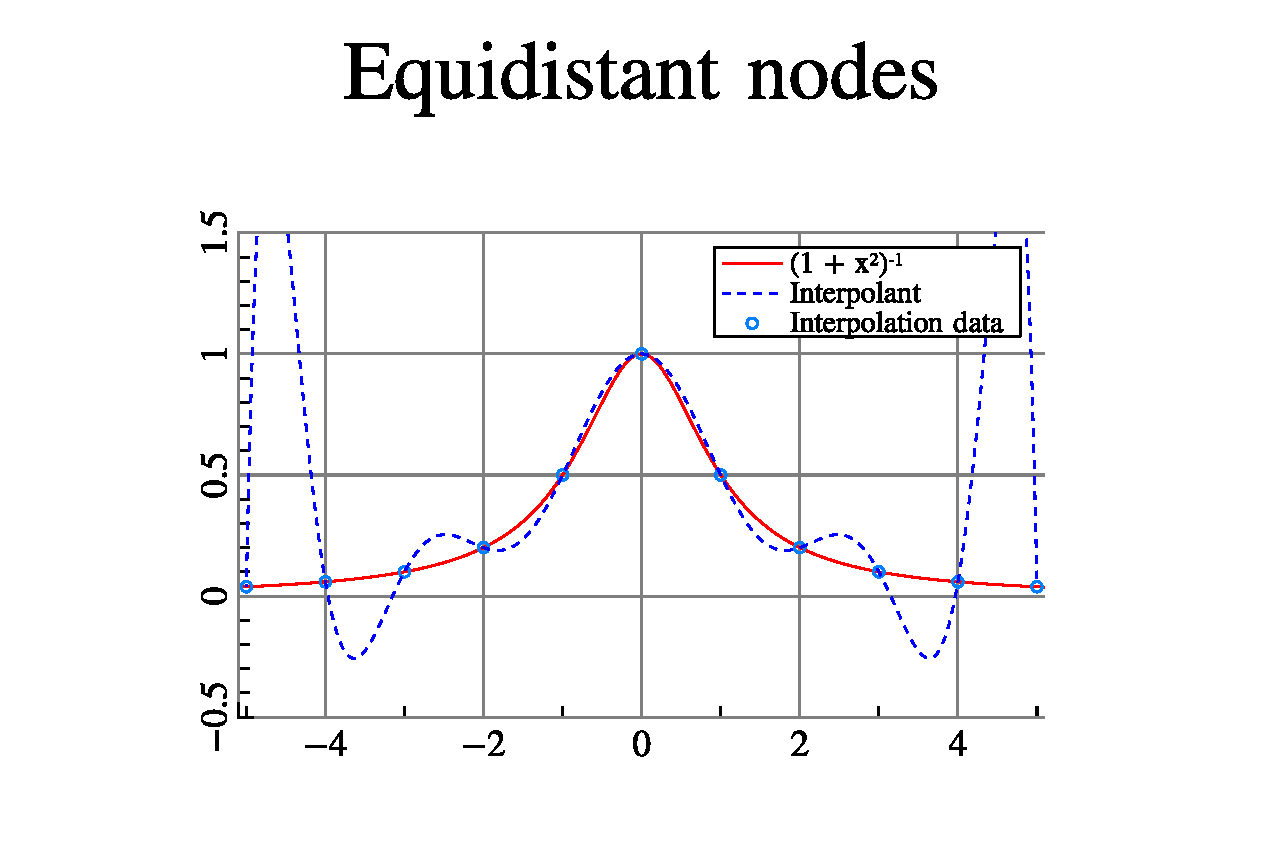
\includegraphics[width=0.5\textwidth]{../../interpolation/node-comparison/build/intp-equi.eps}}
  \subfigure{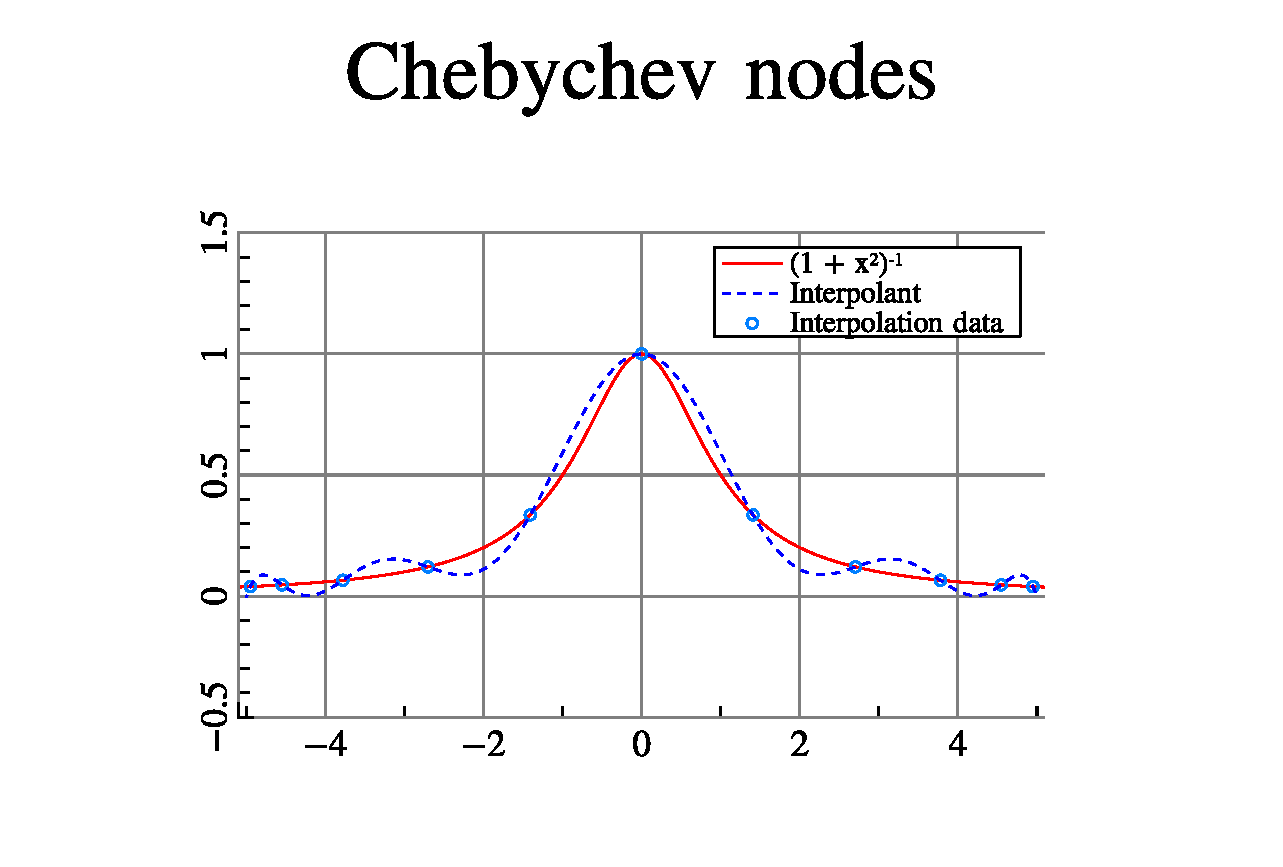
\includegraphics[width=0.5\textwidth]{../../interpolation/node-comparison/build/intp-cheb.eps}}
     \caption{Global polynomial interpolation}
\end{figure}

\begin{figure}[h]
  \centering
  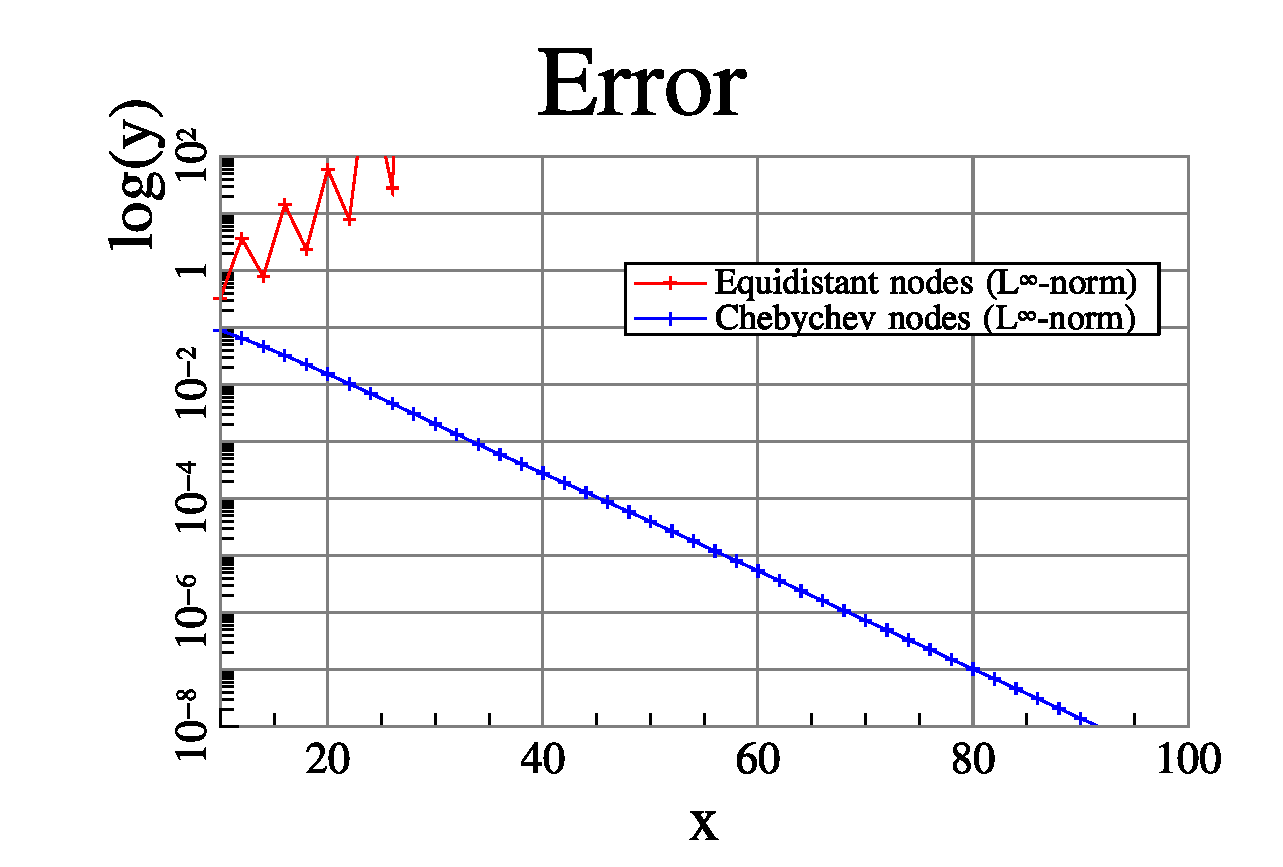
\includegraphics[width=0.7\textwidth]{../../interpolation/node-comparison/build/error.eps}
  \caption{Error of the interpolant}
\end{figure}

The code is divided into the \texttt{library} with the interpolation function and the \texttt{main} function, where the interpolation
function is called.\\
Main:
\begin{minted}[mathescape,linenos,fontsize=\footnotesize]{c++}
include <iostream>
# include <cmath>
# include <vector>
# include "interpol.hpp" // interpol already includes Eigen/Dense
# include <mgl2/mgl.h>

double interpol(Eigen::VectorXd t, mglGraph* gr = 0)
{
  Eigen::VectorXd y = (1/(1 + t.array()*t.array())).matrix();

  Interpol intp(t, y);

  long N = 500;
  Eigen::VectorXd t_intp = Eigen::VectorXd::LinSpaced(N, -5, 5);
  Eigen::VectorXd y_intp(t_intp.size());
  for (long i = 0; i < N; ++i)
    y_intp(i) = intp(t_intp(i));

  if (gr != 0){
    // plot interpolation
    mglData td(t.data(), t.size());
    mglData yd(y.data(), y.size());
    mglData td_intp(t_intp.data(), t_intp.size());
    mglData yd_intp(y_intp.data(), y_intp.size());

    gr->SetRanges(-5.1,5.1,-0.5,1.5);
    gr->Axis();
    gr->Gird("","h");
    gr->FPlot("1/(1+x^2)","r");
    gr->Plot(td, yd, " no");
    gr->Plot(td_intp, yd_intp, "b;");

    gr->AddLegend("\\(1 + x^2)^{-1}", "r");
    gr->AddLegend("Interpolant", "b;");
    gr->AddLegend("Interpolation data", " no");
    gr->Legend();
  }
  // compute maximal error
  double max_err = ((1/(1 + t_intp.array()*t_intp.array())).matrix() - y_intp).maxCoeff();
  return max_err;
}

int main()
{

  /** Plotting for n = 10 nodes **/
  long n = 10;
  // equidistant nodes
  Eigen::VectorXd t_equi = Eigen::VectorXd::LinSpaced(n + 1, -5, 5);
  // chebychev nodes
  Eigen::VectorXd t_cheb(n + 1);
  const double pi = 4*atan(1);
  for (int i = 0; i <= n; ++i)
    t_cheb(i) = -5 + 5*(cos((2*i + 1)*pi/(2*n + 2)) + 1);

  mglGraph gr_equi, gr_cheb;
  gr_equi.Title("Equidistant nodes");
  interpol(t_equi, &gr_equi);
  gr_equi.WriteEPS("intp-equi.eps");

  gr_cheb.Title("Chebychev nodes");
  interpol(t_cheb, &gr_cheb);
  gr_cheb.WriteEPS("intp-cheb.eps");

  /** Plotting error **/
  long N = 100;

  
  // computing error
  std::vector<double> err_equi, err_cheb, evals;
  err_equi.reserve(N/2);
  err_cheb.reserve(N/2);
  evals.reserve(N/2);
  
  for(long n = 10; n < N; n += 2){
    evals.push_back(n);
    // equidistant nodes
    Eigen::VectorXd t_equi = Eigen::VectorXd::LinSpaced(n + 1, -5, 5);
    
    // chebychev nodes
    Eigen::VectorXd t_cheb(n + 1);
    for (int i = 0; i <= n; ++i)
      t_cheb(i) = -5 + 5*(cos((2*i + 1)*pi/(2*n + 2)) + 1);

    err_equi.push_back(interpol(t_equi));
    err_cheb.push_back(interpol(t_cheb));
  }

  // preparing data for plot
  mglData evals_data(evals.data(), evals.size());
  mglData cheb_data(err_cheb.data(), err_cheb.size());
  mglData equi_data(err_equi.data(), err_equi.size());

  // plotting
  mglGraph gr_error;
  gr_error.Title("Error");
  gr_error.SetRanges(10, N, 1e-8, 1e2);
  gr_error.SetFunc("","lg(y)");
  gr_error.Label('x', "x", 0);
  gr_error.Label('y', "log(y)", 0);

  gr_error.Plot(evals_data, equi_data, "r-+");
  gr_error.Plot(evals_data, cheb_data, "b-+");

  gr_error.AddLegend("Equidistant nodes (L^{\\infty}-norm)", "r-+");
  gr_error.AddLegend("Chebychev nodes (L^{\\infty}-norm)", "b-+");
  gr_error.Legend(1,0.8);

  gr_error.Axis();
  gr_error.Grid("","h");

  gr_error.WriteEPS("error.eps");
    

  return 0;
}
\end{minted}

Library (Declaration):
\begin{minted}[mathescape,linenos,fontsize=\footnotesize]{c++}
# ifndef INTERPOL_HPP
# define INTERPOL_HPP

# include <Eigen/Dense>

class Interpol {
  public:
    Interpol(Eigen::VectorXd& t, Eigen::VectorXd& y);
    double operator()(double x);

  private:
    Eigen::VectorXd t_;
    Eigen::VectorXd y_;
    Eigen::VectorXd lambda_;
};

# endif
\end{minted}

Library (Implementation):
\begin{minted}[mathescape,linenos,fontsize=\footnotesize]{c++}
# include <interpol.hpp>
# include <algorithm>
# include <numeric> // accumulate
# include <functional> // mulitplies

Interpol::Interpol(Eigen::VectorXd& t, Eigen::VectorXd& y)
{
  assert(t.size() == y.size()); // should be implemented with try and catch
  const long n = t.size() - 1; // t = t_0,... ,t_n -> size = n + 1
  Eigen::VectorXd lambda = Eigen::VectorXd::Zero(n + 1);

  for (long i = 0; i < n + 1; ++i){
    std::vector<double> T;
    T.reserve(n);
    for (long j = 0; j < n + 1; ++j){
      if (i != j)
        T.push_back(t(i) - t(j)); 
    }

    // following line computes the product of the elements in T
    double T_prod = std::accumulate(T.begin(), T.end(), 1.0, std::multiplies<double>());
    lambda(i) = 1./T_prod;
  }
  t_ = t;
  y_ = y;
  lambda_ = lambda;
}

double Interpol::operator()(double x){
  auto ind_ptr = std::find(t_.data(), t_.data() + t_.size(), x);
  int ind = ind_ptr - t_.data(); // get index as number
  // if x has the same value as a node we must avoid division by 
  // zero and return the value at the node
  if (ind_ptr != t_.data() + t_.size())
    return y_(ind);
  // else use baryzentric formula
  Eigen::VectorXd mu = (lambda_.array()/(x - t_.array())).matrix();
  double result = (mu.array()*y_.array()).sum()/mu.sum();
  return result;
}
\end{minted}

\subsubsection{Natural splines}

\begin{figure}[h]
  \centering
  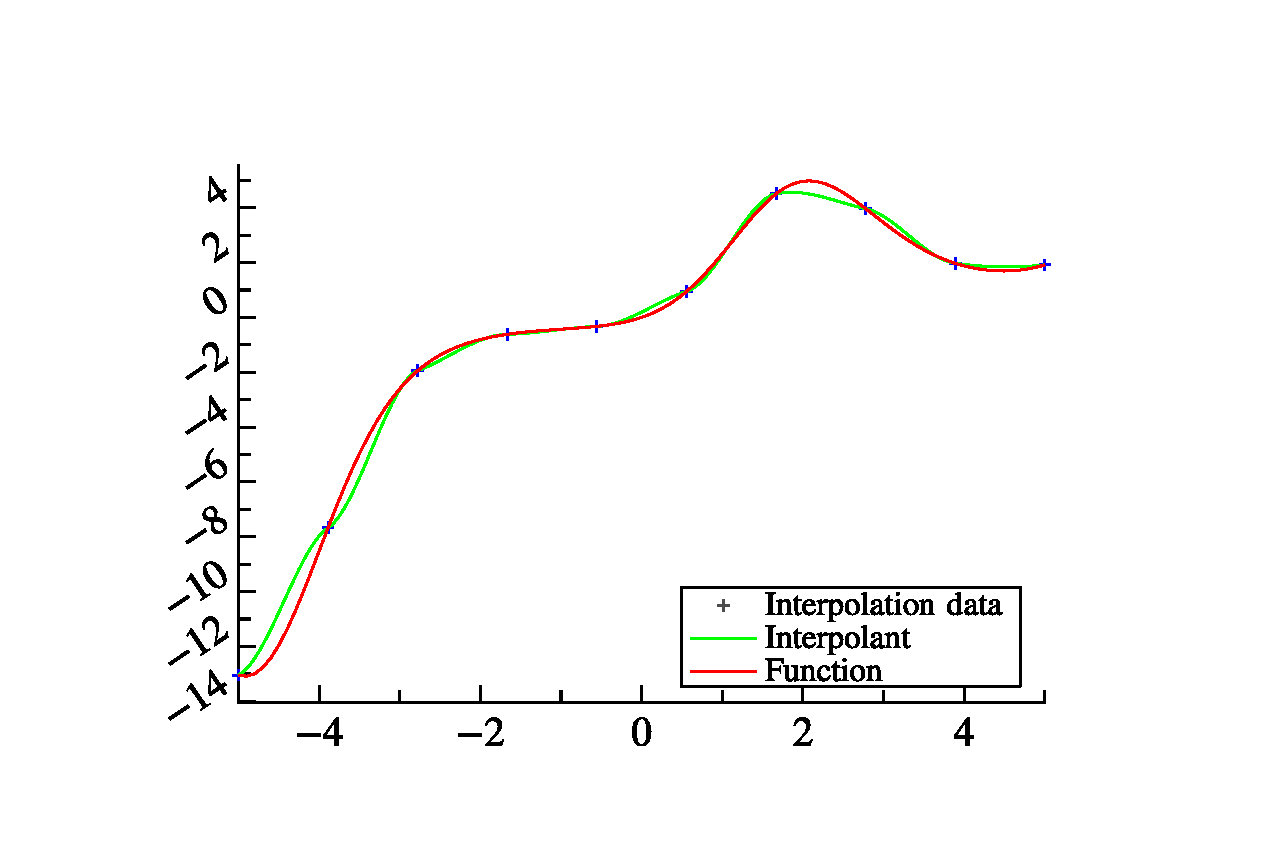
\includegraphics[width=0.7\textwidth]{../../interpolation/cubic-splines/build/interpolation.eps}
\end{figure}

Here the code is also divided in library and main function. \\
Main:
\begin{minted}[mathescape,linenos,fontsize=\footnotesize]{c++}
# include <natcsi.hpp>
# include <Eigen/Dense>
# include <mgl2/mgl.h>
# include <iostream>
# include <fstream>

int main(){
  // build data, function f(t) = t*exp(sin(t))
  Eigen::VectorXd t = Eigen::VectorXd::LinSpaced(10, -5, 5);
  Eigen::VectorXd y = (t.array()*t.array().sin().exp()).matrix();
  NatCSI N(t, y);
  const std::size_t n = 200;
  Eigen::VectorXd t_interp = Eigen::VectorXd::LinSpaced(n, t.minCoeff(), t.maxCoeff());
  Eigen::VectorXd y_interp(n);
  for (std::size_t i = 0; i < n; ++i){
    y_interp(i) = N(t_interp(i));
  }
  // prepare data for plotting
  mglData td, yd, td_interp, yd_interp;
  td.Set(t.data(), t.size()); td_interp.Set(t_interp.data(), t_interp.size());
  yd.Set(y.data(), y.size()); yd_interp.Set(y_interp.data(), y_interp.size());

  // plot
  mglGraph gr;
  gr.SetRanges(t_interp.minCoeff(), t_interp.maxCoeff(), y_interp.minCoeff() - 1, 
    y_interp.maxCoeff() + 1);
  gr.Axis();
  gr.Plot(td, yd, " +"); // interpolation data
  gr.Plot(td_interp, yd_interp, "g"); // interpolant
  gr.FPlot("x*exp(sin(x))", "r"); // function
  
  gr.AddLegend("Interpolation data", " +");
  gr.AddLegend("Interpolant", "g");
  gr.AddLegend("Function", "r");
  gr.Legend(1,0);

  gr.WriteEPS("interpolation.eps");


  return 0;
}
\end{minted}

Library (Declaration):
\begin{minted}[mathescape,linenos,fontsize=\footnotesize]{c++}
# ifndef NATCSI_HPP
# define NATCSI_HPP

# include <Eigen/Dense>

class NatCSI {
  public:
    NatCSI(const Eigen::VectorXd& t, const Eigen::VectorXd& y);
    double operator() (double x) const;

  private:
    Eigen::MatrixXd t_;
    Eigen::VectorXd y_;
    Eigen::VectorXd c_;
};

# endif
\end{minted}

Library (Implementation):
\begin{minted}[mathescape,linenos,fontsize=\footnotesize]{c++}
# include "natcsi.hpp"
# include <Eigen/Dense>
# include <Eigen/Sparse> 
# include <Eigen/SparseCholesky>
# include <vector>
# include <algorithm>
# include <cassert>

// PRE: sorted vector of t and corresponding interpolation values y
// POST: create object of NatCSI
NatCSI::NatCSI(const Eigen::VectorXd& t, const Eigen::VectorXd& y)
: t_(t), y_(y) 
{
  assert(t.size() == y.size());
  const std::size_t n = t.size() - 1; // t = t0, ..., tn -> #t = n+1
  // build helper-definitions
  const Eigen::VectorXd h = t.tail(n) - t.head(n); // #h = n 
  const Eigen::VectorXd b = (1./h.array()).matrix(); // #b = n
  const Eigen::VectorXd a = 2*(b.head(n-1) + b.tail(n-1));
  const Eigen::VectorXd diff_y = y.tail(n) - y.head(n);
  Eigen::VectorXd rhs_constr = (diff_y.array()/h.array()/h.array()).matrix();
  
  // build rhs
  Eigen::VectorXd rhs = Eigen::VectorXd::Zero(n + 1);
  rhs.head(n) = rhs_constr;
  // need to save it temporarily otherwise Eigen starts overwriting 
  // the old vector while we still need it
  Eigen::VectorXd rhs_tail_tmp = rhs.tail(n); 
  rhs.tail(n) = rhs_tail_tmp + rhs_constr;

  // build system matrix
  typedef Eigen::Triplet<double> T;
  std::vector<T> triplets;
  triplets.reserve(3*(n + 1) - 2);

  // first row:
  triplets.push_back( T(0, 0, 2*b(0)) );
  triplets.push_back( T(0, 1, b(0)) );

  // rows 2 to n:
  for (std::size_t i = 1; i < n; ++i){
    triplets.push_back( T(i, i, a(i - 1)) );
    triplets.push_back( T(i, i - 1, b(i - 1)) );
    triplets.push_back( T(i, i + 1, b(i)) );
  }

  // last row:
  triplets.push_back( T(n, n - 1, b(n - 1)) );
  triplets.push_back( T(n, n, b(n - 1)) );

  Eigen::SparseMatrix<double> sysmat(n + 1, n + 1);
  sysmat.setFromTriplets(triplets.begin(), triplets.end());

  // solve LSE
  Eigen::SimplicialLDLT<Eigen::SparseMatrix<double>> solver;
  solver.analyzePattern(sysmat);
  solver.factorize(sysmat);
  c_ = solver.solve(rhs);
}

// PRE: x in between t_0 and t_end
double NatCSI::operator() (double x) const{
  // find out between which nodes x is
  unsigned int index;
  // the case of x being equal to the last node must be 
  // handled separately because the find_if will fail due to the "<"
  if (x == t_(t_.size() - 1)){
    return y_(t_.size() - 1);
  }
  else
  {
    auto f = [x](double node){ return x < node; };
    auto index_pointer = std::find_if(t_.data(), t_.data() + t_.size(), f);
    index = index_pointer - t_.data();
  }
  double h = t_(index) - t_(index - 1);
  x = (x - t_(index - 1))/h;
  double a1 = y_(index) - y_(index - 1);
  double a2 = a1 - h*c_(index - 1);
  double a3 = h*c_(index) - a1 - a2;
  double s =  y_(index - 1) + (a1 + (a2 + a3*x)*(x - 1))*x;
  return s;
}
\end{minted}


\subsection{Newton's method}

This example is about convergence of Newton's method for 
\begin{align}
  z^3 - 1 = 0, \text{  } z \in \mathbb{C}
\end{align}
The following tile plot shows to which of the three roots the method convergence with a given start value. 
The Julia set is the number of points for which the method does not converge. 

\begin{figure}[h]
  \centering
  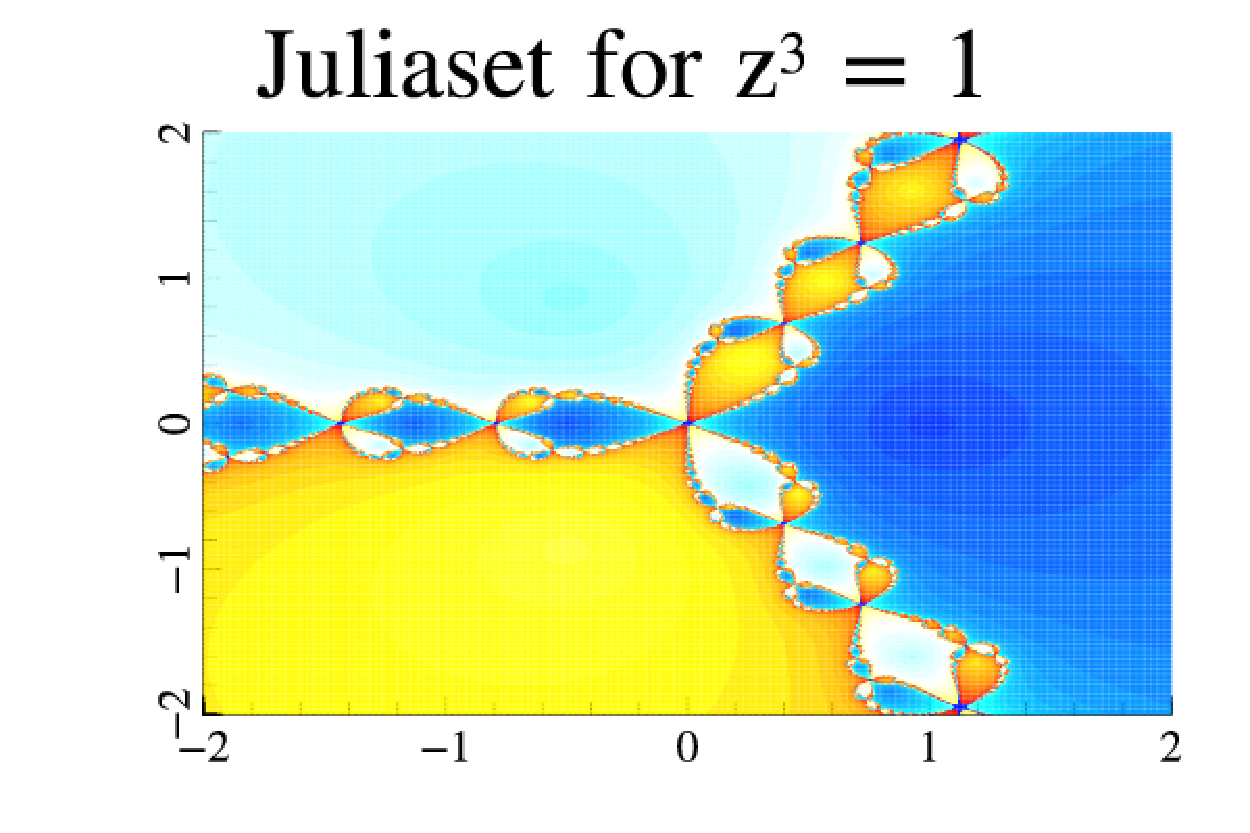
\includegraphics[width=0.7\textwidth]{../../juliaset/set.pdf}
\end{figure}

Code:
\begin{minted}[mathescape,linenos,fontsize=\footnotesize]{c++}
# include <Eigen/Dense>
# include <iostream>
# include <mgl2/mgl.h> 
# include "grid.hpp"

typedef Eigen::VectorXd Vec;
typedef Eigen::MatrixXd Mat;


// define F and its derivative 
class F {
  public:
   Vec operator()(Vec& x)
   {
     Vec fx(2);
     fx << x(0)*x(0)*x(0) - 3*x(0)*x(1)*x(1) - 1,
           3*x(0)*x(0)*x(1) - x(1)*x(1)*x(1);
     return fx;
   }
};

class DF {
  public:
  Mat operator()(Vec& x)
  {
    Mat dfx(2,2);
    dfx <<  3*x(0)*x(0) - 3*x(1)*x(1),
            -6*x(0)*x(1),
            6*x(0)*x(1),
            3*x(0)*x(0) - 3*x(1)*x(1);
    return dfx;
  }
};

int main()
{
  // exact roots of f(z) = z^3 - 1, z \in C
  Vec z1(2), z2(2), z3(2);
  z1 << 1, 0;
  z2 << -0.5, 0.5*std::sqrt(3);
  z3 << -0.5, -0.5*std::sqrt(3);
  const unsigned int maxit = 20;
  const double tol = 1e-4;
  const unsigned int N = 500;
  Vec x = Vec::LinSpaced(N, -2, 2);

  std::pair<Mat, Mat> Grid = meshgrid(x, x);
  Mat X = Grid.first;
  Mat Y = Grid.second;

  Vec C = Vec::Ones(X.size());
  
  F Func; DF Jac;
  for (int i = 0; i < X.size(); ++i){
    Vec v(2); v << *(X.data() + i), *(Y.data() + i);

    // newton iteration
    for (unsigned int k = 1; k <= maxit; ++k){
      v -= Jac(v).lu().solve(Func(v));

      // termination criterium: stop when close to one of the roots
      if ((v - z1).norm() < tol){
        C(i) = 1 + k;
        break;
      }
      else if ((v - z2).norm() < tol){
        C(i) = 1 + k + maxit;
        break;
      }
      else if ((v - z3).norm() < tol){
        C(i) = 1 + k + 2*maxit;
        break;
      }
    }
  }


  // normalize results for plot
  C = (C.array()/double(C.maxCoeff())).matrix();

  mglData Xd(X.rows(), X.cols(), X.data());
  mglData Yd(Y.rows(), Y.cols(), Y.data());
  mglData Cd(X.rows(), X.cols(), C.data());

  mglGraph gr;
  gr.SubPlot(1,1,0,"<_");
  gr.SetRanges(-2,2,-2,2);
  gr.SetRange('c', 0, 1);
  gr.Title("Juliaset for \\z^3 = 1");
  gr.Axis();
  gr.Colorbar("bcwyr");
  gr.Tile(Xd, Yd, Cd, "bcwyr");
  gr.WriteEPS("set.eps");

  return 0;
}

\end{minted}

The used library \texttt{grid.hpp}:
\begin{minted}[mathescape,linenos,fontsize=\footnotesize]{c++}
# ifndef GRID_HPP
# define GRID_HPP

# include <Eigen/Dense>

typedef Eigen::MatrixXd Mat;
typedef Eigen::VectorXd Vec;
std::pair<Mat, Mat> meshgrid(Vec& a, Vec& b)
{
  long m = a.size();
  long n = b.size();
  Mat X(n,m), Y(n,m);
  for (int i = 0; i < n; ++i)
    X.block(i, 0, 1, m) = a.transpose();
  for (int j = 0; j < m; ++j)
    Y.block(0, j, n, 1) = b;
  return std::pair<Mat,Mat>(X,Y);
}

# endif
\end{minted}

\end{document}
